We run the algorithm 5 times for each number of processors on the image shown above, up to 192 processors.
We averaged the 5 runs.
Below the total runtime for each number of processors:
\begin{figure}[H]
  \centering
  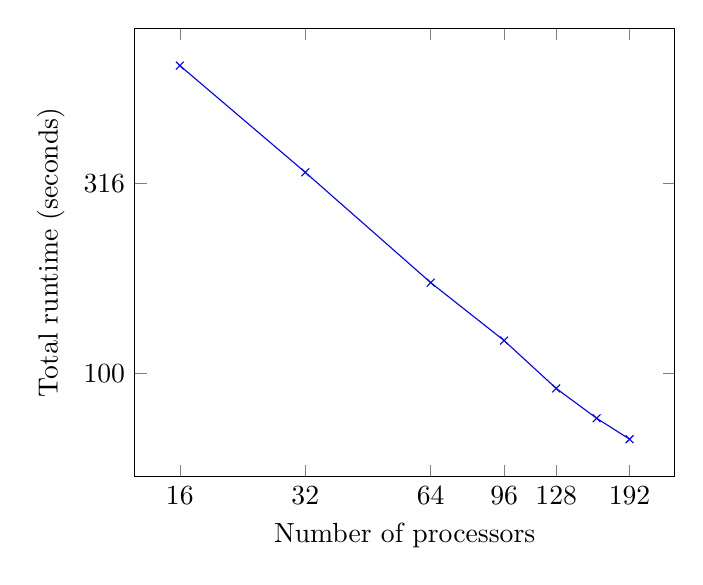
\begin{tikzpicture}
 \begin{axis}[
  xlabel=Number of processors,
  xtick={16, 32, 64, 96, 128, 192},
  xmode=log,
  ymode=log,
  log ticks with fixed point,
  ylabel=Total runtime (seconds)]
   \addplot[color=blue, mark=x] coordinates {
    %(1, )
    %(2, )
    %(4, )
    %(8, )
    (16, 646.344379)
    (32, 338.1412974)
    (64, 173.1325498)
    (96, 121.8080638)
    (128, 91.1042946)
    (160, 76.0524958)
    (192, 66.9623342)
   };
 \end{axis}
\end{tikzpicture}

  \caption{Total runtime of the algorithm with entire matrix computation.}
\end{figure}

We observe that the runtime decreases significantly with respect to the number of processors.
We can also see that, by doubling the number of processors, we nearly accelerate the runtime by a factor 2.
It is an excellent result since we achieve strong scalability for the entire matrix computation case.
However, some overhead will always be present and the matrix-vector operations necessarily require communication, limiting scalability.
To observe if some parts scale better than others, we compare the proportion of each part:
\begin{figure}[H]
  \centering
  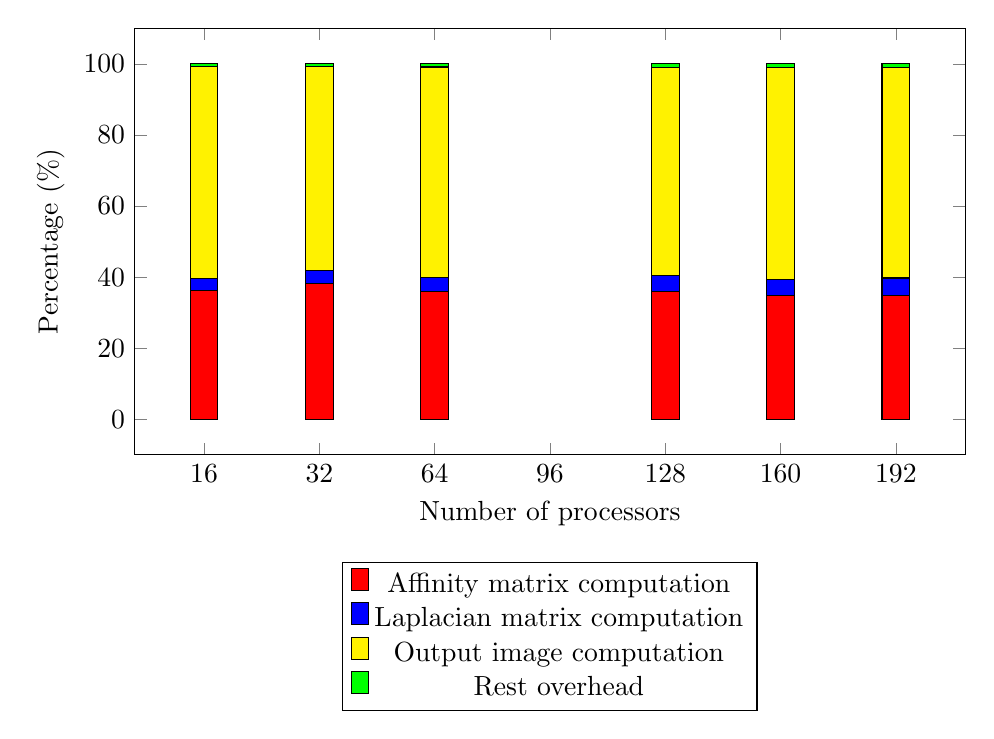
\begin{tikzpicture}
 \begin{axis}[
  ybar stacked,
  height=7cm,
  width=\textwidth,
  xlabel=Number of processors,
  symbolic x coords={
      16, 32, 64, 96, 128, 160, 192
  },
  xtick=data,
  legend style={
   at={(0.5, -0.25)},
   anchor=north
  },
  ylabel={Percentage (\%)}]
  \addplot[ybar, fill=red] plot coordinates {
   (16, 36.11)
   (32, 38.28)
   (64, 36.03)
   (96, 0)
   (128, 36.04)
   (160, 34.73)
   (192, 34.76)};
  \addplot[ybar, fill=blue] plot coordinates {
   (16, 3.62)
   (32, 3.59)
   (64, 3.90)
   (96, 0)
   (128, 4.49)
   (160, 4.71)
   (192, 5)};
  \addplot[ybar, fill=yellow] plot coordinates {
   (16, 59.49)
   (32, 57.32)
   (64, 59.18)
   (96, 0)
   (128, 58.47)
   (160, 59.57)
   (192, 59.21)};
  \addplot[ybar, fill=green] plot coordinates {
   (16, 0.78)
   (32, 0.81)
   (64, 0.89)
   (96, 0)
   (128, 1)
   (160, 1)
   (192, 1.03)};
  \legend{
   Affinity matrix computation,
   Laplacian matrix computation,
   Output image computation,
   Rest overhead}
 \end{axis}
\end{tikzpicture}

  \caption{Proportion of each step in the total execution of the algorithm with entire matrix computation.}
\end{figure}

We see that the proportion of each part remains the same over the increase of processors, meaning that the three main parts scale equivalently.
However, when allocating an excessive amount of processors to this task compared to the input size, we may observe an increase of the runtime because we spend most time on communication overhead.

Overall, computing the entire matrices scales well because we only have matrix-matrix and matrix-vector products.
With an appropriate cluster, those scale nicely.
We now consider larger inputs, which require approximation and introduces some linear algebra which might slow down the process.
